\documentclass{beamer}
\usepackage{pgfpages}
\usepackage{newtxtext,newtxmath} %time new roman
%\setbeameroption{show notes}
%\setbeameroption{show notes on second screen=right}
\usetheme{Warsaw}
\usepackage[french]{babel}

\usepackage{tikz}
\pgfdeclareimage[height=0.5cm]{le-logo}{}
%\setbeamertemplate{footline}[frame number]
%Set number slide 

\usepackage[backend=biber]{biblatex}
%\usepackage[backend=biber, style=chem-acs]{biblatex}
\addbibresource{presentation.bib} 
\bibliography{Skin Cancer Detection}
\setbeamertemplate{bibliography item}[triangle]

\usepackage{multirow}% row fusion
\usepackage{array} % column fusion
\usepackage{xfrac} % small fractions
\usepackage{adjustbox}
\usepackage{listings}
\usepackage{color}
\definecolor{gray}{rgb}{0.4,0.4,0.4}
\definecolor{darkblue}{rgb}{0.0,0.0,0.6}
\definecolor{cyan}{rgb}{0.0,0.6,0.6}
 \titlegraphic{\vspace{-1cm}
      
\includegraphics[width=2.5cm]{images/paris8_1}\hspace*{4.75cm}~%
      \hfill
      
\includegraphics[width=2.5cm]{images/logo}
}
\setbeamertemplate{frametitle}{\nointerlineskip  
    \begin{beamercolorbox}[wd=\paperwidth,ht=2.75ex,dp=1.375ex]{frametitle}
        \hspace*{2ex}\insertframetitle \hfill {\small\insertframenumber/\inserttotalframenumber} \hspace*{1ex}%
    \end{beamercolorbox}}

\usecolortheme{wolverine}
\setbeameroption{hide notes} % Only slides


%%%%%%%%%%%%%%%%%%%%%%%%%%%
\title[Skin Cancer Detection Using Convolutional Neural Network] 
{Skin Cancer Detection Using Convolutional Neural Network}
%\subtitle {ne compléter que si l'article possède un sous-titre}
\author[Komlan Dantodji] 
{Komlan Jean-Marie DANTODJI}

\institute[]
{
  Etudiant en M1 Big Data
  \and
  Université Paris 8}
\date{December 17, 2020}


\begin{document}
\begin{frame}
  \titlepage
\end{frame}

\begin{frame}{Summary}
  \tableofcontents
\end{frame}

\section{Introduction}
\begin{frame}{Skin Cancer}
\begin{figure}[H]
    \includegraphics[width=8cm,height=4cm]{images/cancer.png}
    \caption{ Skin Cancer: From Google}
    \label{fig:L1}
\end{figure}
\end{frame}

\section{Issue}
\begin{frame}{Issue}
\begin{itemize}
		\item Find a way to diagnostic cancerous cells from image 
		\item Extract features from the image
		\item Apply Convolutional Neuronal Network to layers 
\end{itemize}
\end{frame} 

\section{Background and Related works}
\begin{frame}{Background and Related works 1/2}
\begin{itemize}
		\item Robert Amelard et al:\\
		Illumination correction and feature extraction framework based on high level intuitive feature implemented on skin images.
		\item A. Goshtasbya D. Rosemanb S. Binesb C. Yuc A. Dhawand A. Huntleye L. Xua:\\
		Back-propagation neural network (BNN) and Auto-associative neural network.
\end{itemize}
\end{frame} 
\begin{frame}{Background and Related works 2/2}
\begin{itemize}
		\item Ramteke et al. : \\
		ABCD standard to recognize skin malignant growth
		\item Sibi Salim RB Aswin, J Abdul Jaleel. 2013: \\
		ANN Classifier using MATLAB for Skin Cancer Detection.
\end{itemize}
\end{frame} 


\section{Input image and Dataset}
\begin{frame}{Input image and Dataset}
\begin{itemize}
		\item Image of patient's body
		\item Dataset of 23907 images from ISIC Archive
\end{itemize}
\end{frame} 
%\begin{frame}{Skin Cancer}
%\end{frame} 
\section{Differents step of detecting cancer in image} 
\begin{frame}{Chart of steps}
\begin{figure}[H]
    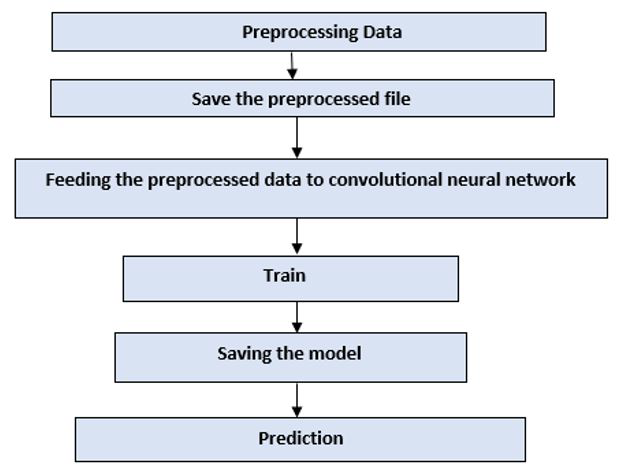
\includegraphics[width=8cm,height=4.5cm]{images/steps.png}
    \caption{[1] Chart display steps of the model CNN, page 255}
    \label{fig:L1}
\end{figure}
\end{frame} 
\begin{frame}{Step 1: Preprocessing Data}
\begin{itemize}
		\item Convert all images to the gray-scale
		\item Resize images to reduce time of processing
\end{itemize}
\end{frame} 

\begin{frame}{Step 2: Save the preprocessed file}
\begin{itemize}
		\item  Binary labels: benign and malignant
		\item Classify each image of dataset to his class
\end{itemize}
\end{frame} 

\begin{frame}{Step 3: Feeding the preprocessed data to CNN 1/3}
\begin{figure}[H]
    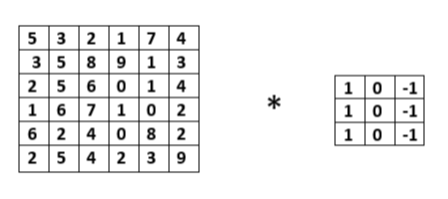
\includegraphics[width=7cm,height=3cm]{images/convolution.png}
    \caption{[1] Gray-scale Image 6x6 and the 3x3 filter, page 256}
    \label{fig:L1}
\end{figure}
$$ \sum_{i=0}^{m-1}\sum_{i=0}^{m-1} X_{(n-i)(n-j)}Y_{(i+1)(j+1)}    (1)$$
\end{frame} 

\begin{frame}{Step 3: Result of Pooling 2/3}
We get the result as follow:
\begin{figure}[H]
    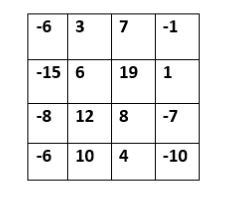
\includegraphics[width=7cm,height=4cm]{images/pooling.png}
    \caption{[1] 4x4 image after applying 3x3 filter to the gray-scale image, page 257}
    \label{fig:L1}
\end{figure}
\end{frame} 

\begin{frame}{Step 3: Max Pooling 3/3}
Extract more features
\begin{figure}[H]
    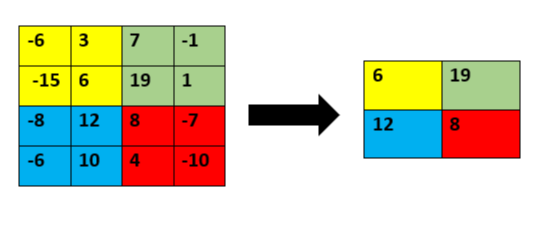
\includegraphics[width=7cm,height=3cm]{images/maxpooling.png}
    \caption{[1] Result after applying max pooling, page 257}
    \label{fig:L1}
\end{figure}
\end{frame} 

\begin{frame}{Steps 4 and 5: Train and save the model}
\begin{itemize}
		\item  Train the model 200 times of epoch
		\item Save the model 
\end{itemize}
\end{frame} 

\begin{frame}{Step 6: Test and predict cancer}
\begin{itemize}
		\item  Feed image to the model for prediction
\end{itemize}
$$ Recall = \frac{TruePositive}{Positive }  (2)$$
$$ Specificity = \frac{TrueNegative}{Negative} (3)$$
$$ Precision = \frac{TruePositive}{TruePositive + FalsePositive} (4)$$
$$ Score = \frac{2*Precision*Recall}{Precision+Recall} (5)$$
\end{frame} 


\section{Discussions and results}
\begin{frame}{Neurons vs accuracy}
\begin{figure}[H]
    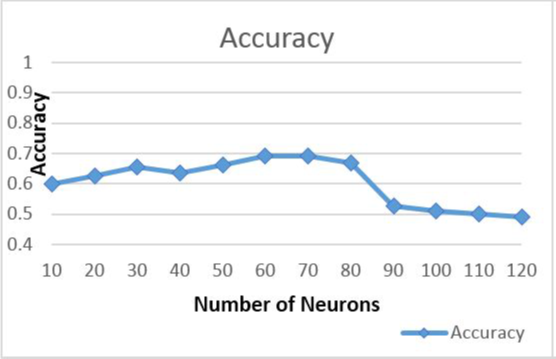
\includegraphics[width=9cm,height=5cm]{images/discuss_1.png}
    \caption{[1] Neurons vs accuracy, page 257}
    \label{fig:L1}
\end{figure} 
\end{frame}

\begin{frame}{Iteration vs loss}
\begin{figure}[H]
    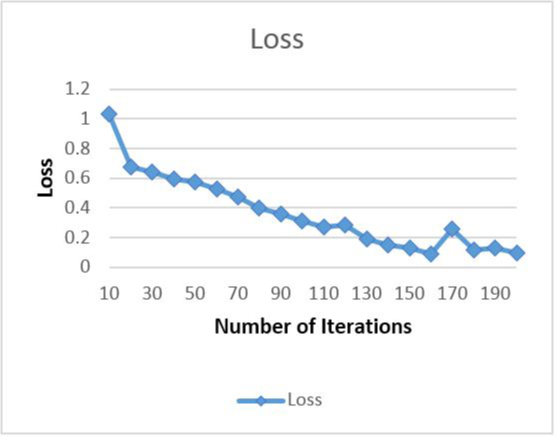
\includegraphics[width=9cm,height=5cm]{images/discuss_2.png}
    \caption{[1] Iteration vs loss, page 258}
    \label{fig:L1}
\end{figure} 
\end{frame}

\begin{frame}{Iteration vs accuracy}
\begin{figure}[H]
    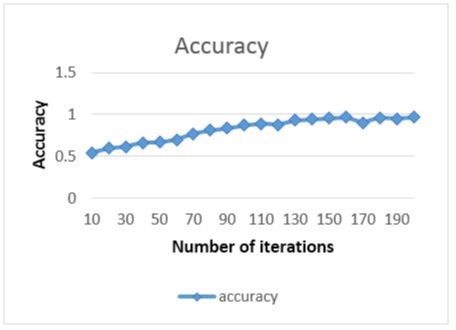
\includegraphics[width=9cm,height=5cm]{images/discuss_3.png}
    \caption{[1] Iteration vs accuracy, page 258}
    \label{fig:L1}
\end{figure} 
\end{frame}

\begin{frame}{Iteration vs Mean Square Error}
\begin{figure}[H]
    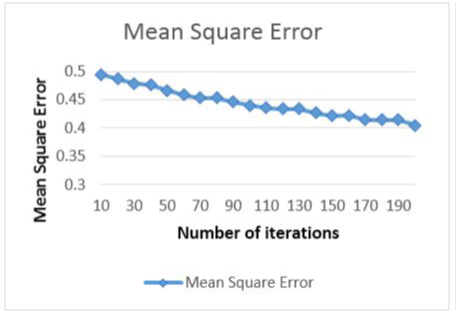
\includegraphics[width=9cm,height=5cm]{images/discuss_4.png}
    \caption{[1] Iteration vs Mean Square Error, page 258}
    \label{fig:L1}
\end{figure} 
\end{frame}

\begin{frame}{Results}
With this model using ISIC archive dataset we get the the result 
$$Recall = 0.84$$
$$Precision = 0.8325$$
$$Score = 0.8325$$
according to [1].
\end{frame}


\section{Conclusion}
\begin{frame}{Conclusion}
\begin{itemize}
		\item Helps dermatologist to dignostisic early skin cancer 
		\item Hight accuracy with the model CNN
\end{itemize}
\end{frame}

\begin{frame}{Référence}
\renewcommand*{\bibfont}{\footnotesize}
\nocite{bibskin}
\printbibliography
\end{frame}

\begin{frame}
  \begin{block}{}
  \centering
  Thank you for your attention...
  \end{block}
\end{frame}
\end{document}
